\section{实验结果及分析}

\subsection{仿真波形}

使用1+2+\ldots+100累加程序进行行为仿真，仿真时长设置为15000ns，testbench在检测到\texttt{dataadr=0且writedata=5050}时打印``Simulation succeeded''并触发\texttt{\$stop}。仿真在12100ns结束，波形结果如图\ref{fig:wave}所示。

\begin{figure}[htbp]
    \centering
    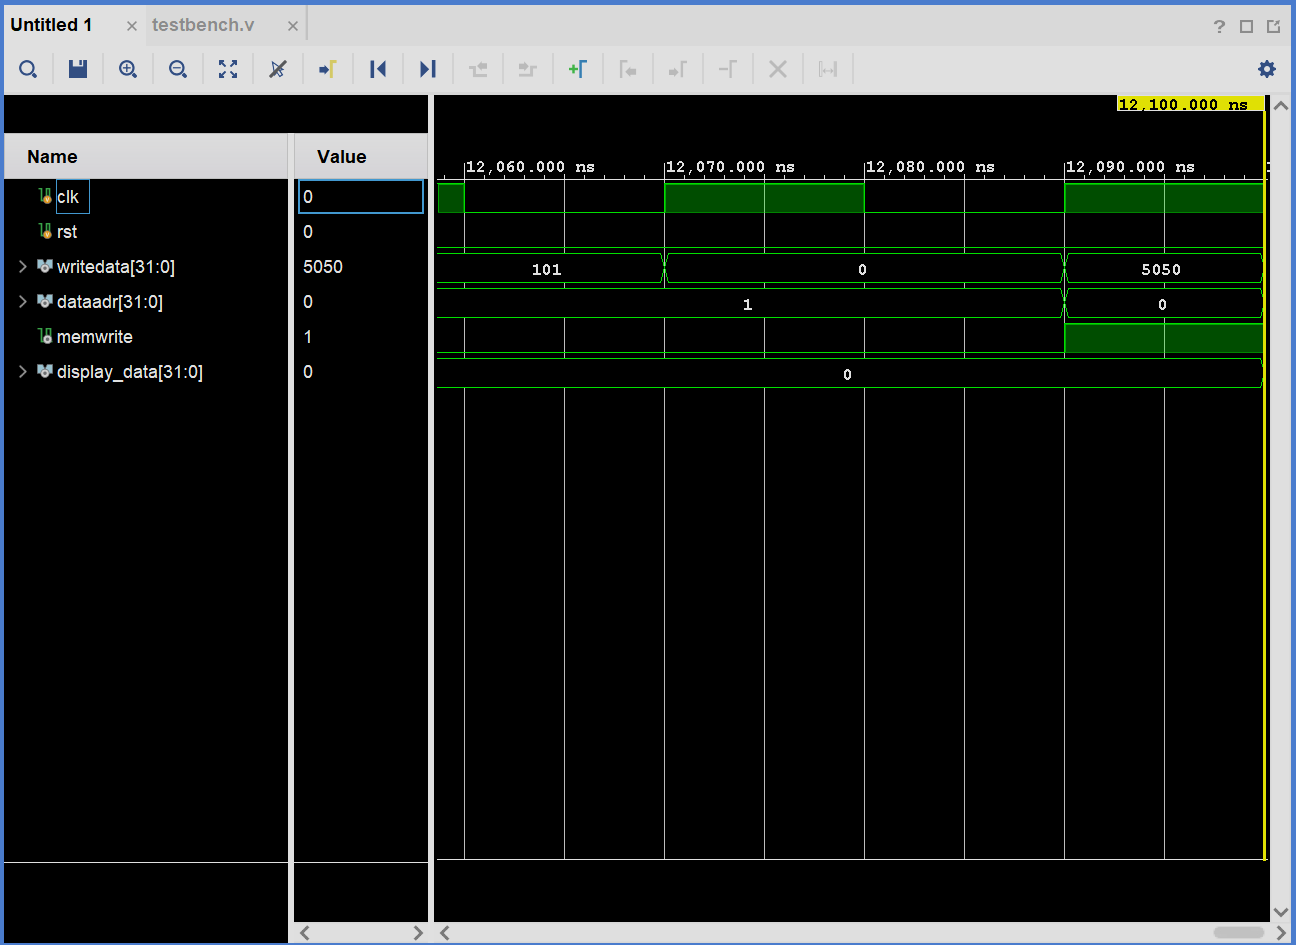
\includegraphics[width=\textwidth]{image/sim_wave.png}
    \caption{累加程序仿真波形（最终时刻：writedata=0x13BA, dataadr=0, memwrite=1）}\label{fig:wave}
\end{figure}

波形重点信号说明：
\begin{itemize}
    \item \texttt{writedata = 0x000013BA}：CPU执行\texttt{sw \$1, 0(\$0)}时输出的写入数据，即累加结果5050；
    \item \texttt{dataadr = 0x00000000}：sw指令的目标地址（mem[0]）；
    \item \texttt{memwrite = 1}：数据存储器写使能；
    \item \texttt{display\_data}：实时反映数据存储器[0]的值，在sw发生时刻从0跳变为5050。
\end{itemize}

\subsection{控制台输出}

Vivado Tcl Console在仿真结束时打印如下信息（见图\ref{fig:console}）：

\begin{figure}[htbp]
    \centering
    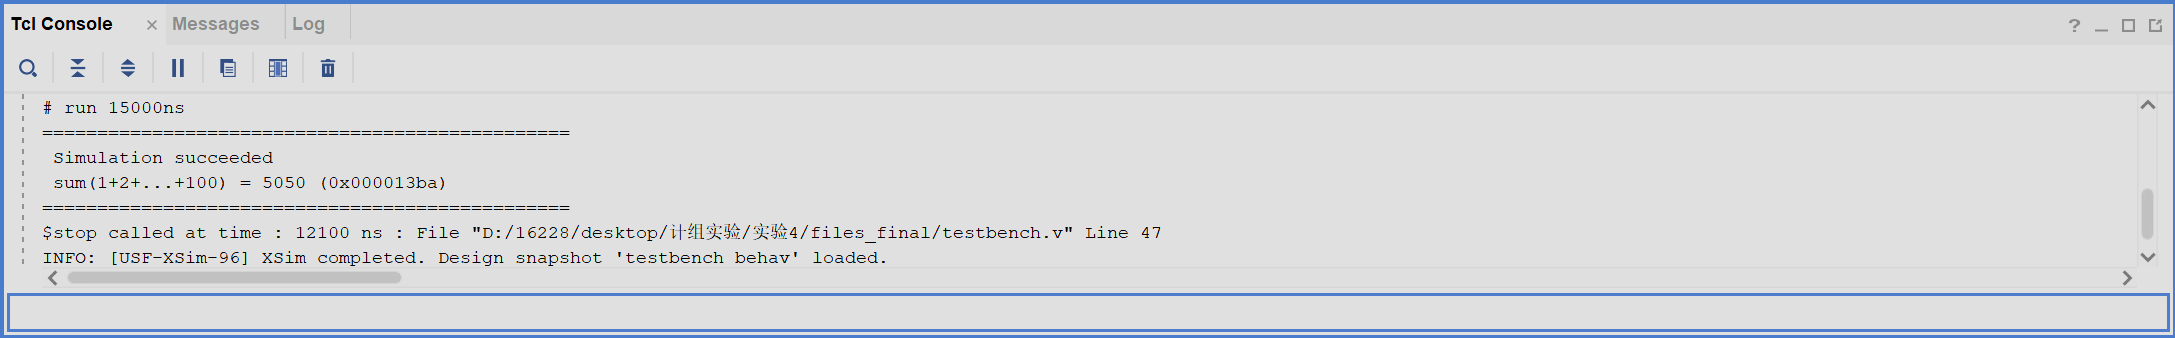
\includegraphics[width=0.85\textwidth]{image/sim_console.png}
    \caption{Vivado Tcl Console仿真结果输出}\label{fig:console}
\end{figure}

输出关键内容：
\begin{verbatim}
================================================
 Simulation succeeded 
 sum(1+2+...+100) = 5050 (0x000013ba)
================================================
$stop called at time : 12100 ns
\end{verbatim}

\subsection{结果分析}

\subsubsection{周期数分析}

总执行周期数 = 12100ns / 20ns = 605个周期。该数值与理论估算吻合：

\begin{itemize}
    \item 流水线初始填充：约5个周期（流水线深度-1+反应时间）；
    \item 3条初始化addi：连续顺序执行，无气泡；
    \item 100次循环 × 每轮5条指令（add、addi、slt、beq、sw）：
    \begin{itemize}
        \item 循环体5条指令本身占5个周期；
        \item beq判断成功跳转回循环开始，需冲刷IF/ID和ID/EX中的2条指令，引入1个气泡（实际损失2拍流水气泡，但下一轮取指即可继续）；
        \item 每轮约6个周期；
    \end{itemize}
    \item 最后一次循环beq不成立，继续往下执行sw，最终触发testbench停止。
\end{itemize}

实际605周期 ≈ 5（启动）+ 3（初始化）+ 100×6（循环）+ 2（sw及之后），略大于估算，差距来自beq成立时的额外气泡和流水线启动空拍，完全在合理范围内。

\subsubsection{与单周期CPU性能对比}

实验三单周期CPU执行同样的累加程序，每条指令1个周期完成，理论上需要约 $3 + 100 \times 5 + 1 = 504$ 个周期。但由于单周期CPU需要将时钟周期拉长到最慢指令的延迟（约40\,ns），单周期CPU实际耗时 $504 \times 40 = 20160$\,ns。

本实验流水线CPU的时钟周期为20\,ns（50\,MHz），605个周期共耗时12100\,ns。\textbf{相比单周期CPU加速比约为1.66倍}，符合流水线理论加速效果（理论上限为流水级数5，受冒险气泡和分支冲刷影响实际加速比小于5）。

\subsubsection{冒险处理正确性验证}

仿真过程中，CPU正确处理了多种典型冒险场景：

\begin{itemize}
    \item \textbf{EX前推}：\texttt{add \$1, \$1, \$2}紧跟\texttt{addi \$1, \$0, 0}和\texttt{addi \$2, \$0, 1}，前者在add执行时已处于WB阶段（WB→EX前推），后者在MEM阶段（MEM→EX前推）；
    \item \textbf{相邻指令前推}：循环中\texttt{slt \$4, \$3, \$2}紧跟\texttt{addi \$2, \$2, 1}，前者读\$2需要从前者的EX前推；
    \item \textbf{beq控制冒险}：每次循环beq成立时，flushD冲刷IF/ID，flushE\_total冲刷ID/EX，避免延迟槽指令错执行；
    \item \textbf{j跳转}：程序末尾\texttt{j 8}进入死循环，jumpD信号正确触发PC跳转和IF/ID冲刷。
\end{itemize}

\subsection{验证结论}

本次实验完整实现了五级流水线MIPS CPU，正确处理了数据冒险和控制冒险。累加测试程序仿真结果5050（0x13BA）与单周期CPU完全一致，流水线吞吐量明显高于单周期实现，达到了设计目标。
